\documentclass{beamer}
\usepackage[utf8]{inputenc}
\usepackage[danish, english]{babel}
\usepackage{beamerthemesplit}
\usepackage{color}

% Math support
\usepackage{amssymb}
\usepackage{amsmath}

\title[OCamlCSP]{
  OCamlCSP - A concurrency library for OCaml
}
\author[Joakim A.]{
  Joakim Ahnfelt-Rønne
}
\institute[DIKU]{
  Datalogisk Institut \\ Københavns Universitet
}
\date{25. august 2009}

\definecolor{kugreen}{RGB}{50,93,61}
\definecolor{kugreenlys}{RGB}{132,158,139}
\definecolor{kugreenlyslys}{RGB}{173,190,177}
\definecolor{kugreenlyslyslys}{RGB}{214,223,216}
\setbeamercovered{transparent}
\mode<presentation> {
 \usetheme{PaloAlto}
 \usecolortheme[named=kugreen]{structure}
 \useinnertheme{circles}
 \usefonttheme[onlymath]{serif}
 \setbeamercovered{transparent}
 \setbeamertemplate{blocks}[rounded][shadow=true]
}
\logo{
\includegraphics[width=1cm]{figures/B_NAT_cmyk.pdf}}

\begin{document}

\frame{
 \titlepage
}

\section[Hvorfor?]{}
\frame{
  \frametitle{Hvorfor?}
  \begin{itemize}
    \item CSP som model for samtidighed:
    \begin{itemize}
      \item Hierakisk processmodel
      \item Synkron beskedudveksling
      \item Passiv venten på flere kanaler samtidig
    \end{itemize}
  \end{itemize}
}
\frame{
  \frametitle{Eksistensberettigelse}
  \begin{itemize}
    \item Flere biblioteker eksisterer allerede:
    \begin{itemize}
      \item C++CSP (C++) 
      \item JCSP (Java)
      \item PyCSP (Python)
      \item CHP (Haskell)
    \end{itemize}
  \end{itemize}
}
\frame{
  \frametitle{Eksistensberettigelse}
  \begin{itemize}
    \item Flere biblioteker eksisterer allerede:
    \begin{itemize}
      \item C++CSP $\leftarrow$ imperativt sprog, objektorienteret design
      \item JCSP $\leftarrow$ ditto
      \item PyCSP $\leftarrow$ ditto
      \item CHP $\leftarrow$ rent funktionelt sprog, monadisk design
    \end{itemize}
  \end{itemize}
}
\frame{
  \frametitle{Eksistensberettigelse}
  \begin{itemize}
    \item Flere biblioteker eksisterer allerede:
    \begin{itemize}
      \item C++CSP $\leftarrow$ imperativt sprog, objektorienteret design
      \item JCSP $\leftarrow$ ditto
      \item PyCSP $\leftarrow$ ditto
      \item CHP $\leftarrow$ rent funktionelt sprog, monadisk design
      \item \textbf{OCamlCSP} 
      \begin{itemize}
        \item Urent funktionelt sprog (sideeffekter)
        \item Traditionelt ML-design (moduler)
        \item I stil med eksisterende OCaml-biblioteker
      \end{itemize}
    \end{itemize}
  \end{itemize}
}


\section[Målsætning]{}
\frame{
  \frametitle{Målsætning}
  \begin{itemize}
    \item Mål
      \begin{itemize}
      \item At bruge processmodellen og kanalerne fra CSP som fundament for et samtidighedsbibliotek
      \item At levere et lille interface der passer ind i stilen for OCamls eksisterende biblioteker
      \end{itemize}
  \end{itemize}
}



\section[Design]{}
\frame{
  \frametitle{Design}
  \begin{itemize}
    \item Hierakisk processmodel 
      \begin{itemize}
        \item Alle processer er en subprocess af en anden process
        \item En subprocess starter altid efter og slutter altid før sin moderprocess
        \item Gør det nemt at overskue hvilke processer der kører et givent sted i programmet
        \item Kræver til gengæld at man tænker sig om når man har brug for at starte processer som reaktion på en udefra kommende hændelse
        \item Emulering af spawn: continutations? ``Kør dette parallelt med resten af programmet.''
      \end{itemize}
  \end{itemize}
}
\frame{
  \frametitle{Design}
  \begin{itemize}
    \item Kanaler: Repræsentation
      \begin{itemize}
        \item Kanaler skal have et virkefelt - ellers er det ikke til at indkapsle dem i en process
        \item Kun let-bindinger og funktioner giver virkefelt i udtryk i OCaml
        \item Vi binder kanaler med let-bindinger, og dermed skal de være data
        \item Vi begrænser ikke hvad der kan sendes over en kanal
      \end{itemize}
  \end{itemize}
}
\frame{
  \frametitle{Design}
  \begin{itemize}
    \item En finurlig konsekvens
      \begin{itemize}
      \item Alle typer data kan sendes over kanaler
      \item Kanaler er data
      \item Ergo kan kanaler sendes over kanaler, som i $\pi$-calculus
      \end{itemize}
  \end{itemize}
}
\frame{
  \frametitle{Design}
  \begin{itemize}
    \item Kanaler
      \begin{itemize}
        \item De fleste biblioteker skelner mellem one-to-one og any-to-any (med flere)
        \item Der er ingen måde statisk at begrænse brugen af en kanal på
        \item Derfor vælger vi kun at tilbyde den mest generelle, any-to-any
      \end{itemize}
  \end{itemize}
}
\begin{frame}[fragile]
  \frametitle{Design}
  \begin{itemize}
    \item Kanaler: Alternation
      \begin{itemize}
        \item CSP har external choice
        \item Både med read og write guards
        \item Nogle biblioteker har kun read guards
        \item Hvorfor er write guards interessante?
        \item Eksempel: Buffer
          \begin{itemize}
            \item Kan skrive når den ikke er tom
            \item Kan læse når den er ikke fuld
            \item Kan både læse og skrive når den hverken er tom eller fuld
          \end{itemize}
\item Uendelig buffer:
\begin{verbatim}
buffer [] = in ? x -> buffer [x]
buffer (x:xs) = ( in ? y -> buffer (x:xs @ [y]) 
                | out ! x -> buffer xs )
\end{verbatim}
      \end{itemize}
  \end{itemize}
\end{frame}
\frame{
  \frametitle{Design}
  \begin{itemize}
    \item Kanaler: Guards
      \begin{itemize}
        \item CSP og Occam har guarded processes
        \item De fleste biblioteker har guards, hvor man manuelt skal tage beslutninger baseret på hvilken guard der er blevet valgt
        \item Guarded processes kombinerer løftet om at udføre en handling med selve handlingen, og eliminerer dermed en fejlkilde
        \item Flere guards på den samme kanal kan optræde i en select
        \item Vores select minder dermed om general choice, bortset fra at der skal være en synlig guard, som i external choice.
      \end{itemize}
  \end{itemize}
}
\frame{
  \frametitle{Design}
  \begin{itemize}
    \item Kanaler: Valg
      \begin{itemize}
        \item Hvis flere guards er klar på samme tid, hvilken en skal så vælges?
        \item Den første i listen? Dette er Occams PRI ALT. Når man har write guards mister konceptet ``den første'' sin mening.
        \item En arbitrær? Dette er Occams ALT. Præcis som i CSP.
        \item En tilfældig? Giver en garanti for at en guard i gennemsnit bliver valgt et antal gange, der er proportionalt med hvor ofte den er klar i forhold til andre guards.
        \item Vi vælger den sidste løsning
      \end{itemize}
  \end{itemize}
}


\section[Eksempler]{}
\begin{frame}[fragile]
  \frametitle{Eksempel: Fibonacci (parallel)}
Ideel notation for \verb|parallel|:

\begin{verbatim}
FibonacciInt (out) =              (* pseudo-code *)
    PrefixInt (1, c4, c1)   ||
    PrefixInt (0, c1, c2)   ||
    Delta2Int (c2, out, c3) ||
    PairsInt (c3, c4)
\end{verbatim}

Kort og tæt på CSP.
\end{frame}
\begin{frame}[fragile]
  \frametitle{Eksempel: Fibonacci (parallel)}
{\tiny
\begin{verbatim}
FibonacciInt (out) =                                               (* pseudo-code *)
    PrefixInt (1, c4, c1)   ||
    PrefixInt (0, c1, c2)   ||
    Delta2Int (c2, out, c3) ||
    PairsInt (c3, c4)
\end{verbatim}
}
\begin{verbatim}
let fibonacciInt out () =         (* actual code *)
  let c1 = Csp.new_channel () in
  let c2 = Csp.new_channel () in
  let c3 = Csp.new_channel () in
  let c4 = Csp.new_channel () in
    Csp.parallel [
      prefixInt 1 c4 c1;
      prefixInt 0 c1 c2;
      delta2Int c2 out c3;
      pairsInt c3 c4
    ]
\end{verbatim}
\end{frame}
\begin{frame}[fragile]
  \frametitle{Eksempel: Proxy (select)}
Ideel notation for \verb|select|:
\begin{verbatim}
(c1 ? x -> ... | c2 ? (y, z) -> ...)
\end{verbatim}
Kort og tæt på CSP.
\end{frame}
\begin{frame}[fragile]
  \frametitle{Eksempel: Proxy (select)}
Ideel notation for \verb|select|:
\begin{verbatim}
(c1 ? x -> ... | c2 ? (y, z) -> ...)
\end{verbatim}
Vores notation:
\begin{verbatim}
Csp.select [
    Csp.read_guard c1 (fun x -> ...);
    Csp.read_guard c2 (fun (y, z) -> ...)
]
\end{verbatim}
\end{frame}
\begin{frame}[fragile]
  \frametitle{Eksempel: Proxy (select)}
\begin{verbatim}
let cache i o d () =
    let rec loop t =
        Csp.select [
            Csp.read_guard i (fun u ->
                (try let n = Table.find u t in
                    Csp.write o (Some n)
                with Not_found -> Csp.write o None);
                loop t
            );
            Csp.read_guard d (fun (u, n) ->
                loop (Table.add u n t)
            );
        ]
    in loop Table.empty
\end{verbatim}
\end{frame}
\begin{frame}[fragile]
  \frametitle{Anvendelse}
  \begin{itemize}
    \item Anvendelse
    \begin{itemize}
      \item Applikationer der indbyder til en samtidig struktur
        \begin{itemize}
          \item Grafiske brugergrænseflader (event-handling)
          \item Servere (en process til hvert request)
        \end{itemize}
      \item I/O-bundene programmer
    \end{itemize}
  \end{itemize}
\end{frame}


\section[Kode]{}
\frame{
  \frametitle{Implementation}
  \begin{itemize}
  \item Alternation
    \begin{itemize}
    \item Select er som de andre bibliotekers priSelect
    \item Bortset fra at vi permuterer listen tilfældigt først
    \item Først tjekkes det om der er nogen der venter på en af kanalerne
    \item Derefter stiller den sig i kø på hver af kanalerne
    \item Ved kommunikation fjerner den sig fra hver kanals kø
    \end{itemize}
  \end{itemize}
}
\frame{
  \frametitle{Implementation}
  \begin{itemize}
  \item Kanaler
    \begin{itemize}
    \item Kanalers state tager udgang i en finite state machine
    \item Men udvider den til et arbitrært antal af ventende processer
    \item Og understøtter poison
    \end{itemize}
\vspace{0.5cm}
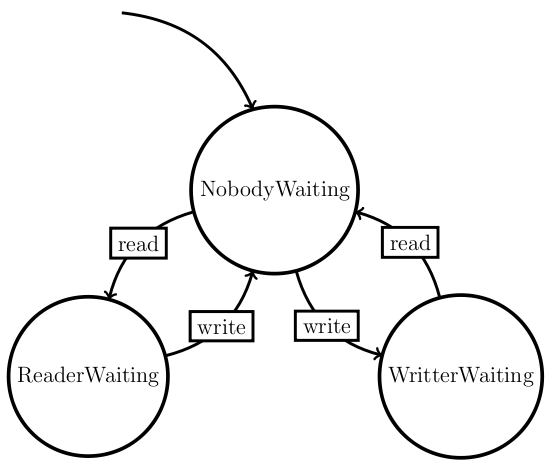
\includegraphics[width=0.4\textwidth]{figures/state.png}
  \end{itemize}
}
\begin{frame}[fragile]
  \frametitle{Implementation}
\begin{verbatim}
let i = Csp.new_channel () in
let o = Csp.new_channel () in
let d = Csp.new_channel () in
let rec loop () =
    let (f, _) = Unix.accept socket in
        let fi = Unix.in_channel_of_descr f in
        let fo = Unix.out_channel_of_descr f in
        Csp.parallel [
            handler fi fo i o d;
            loop   (* run this process in parallel *)
        ]          (* with the rest of the loop    *)
    in Csp.parallel [
        cache o i d;
        loop
    ]
\end{verbatim}
\end{frame}
\frame{
  \frametitle{Implementation}
  \begin{itemize}
    \item But parallel is not tail recursive!
    \item It doesn't seem obvious how to fix this
  \end{itemize}
}
\end{frame}
\frame{
  \frametitle{Implementation}
  \begin{itemize}
    \item Biblioteker med global state er svære at bruge sammen med OCamlCSP
  \end{itemize}
}
\frame{
  \frametitle{Implementation}
  \begin{itemize}
    \item OCaml har ingen garbage collector der kan håndtere samtidighed
    \item Derfor kan et bibliotek bygget på OCamls trådbibliotek ikke understøtte samtidighed på hardware-niveau
    \item Er det overhovedet interessant at basere hardware-samtidighed på en shared-memory model?
    \item Måske kunne man lave en løsning med kommunikation over TCP eller UDP - måske er det ikke praktisk
          på grund af synkroniseringen
  \end{itemize}
}


\section[Spørgsmål]{}
\frame{
  \frametitle{Spørgsmål}
  \begin{itemize}
    \item Slut på præsentationen
  \end{itemize}
}

\frame{
  \frametitle{OCamlCSP versus Occam}
  \begin{itemize}
    \item Differences from Occam
      \begin{itemize}
      \item We have any-to-any channels
      \item Write guarded processes
      \item Channels as data
      \item Channels can be poisoned
      \item We have no way to limit shared state
      \end{itemize}
  \end{itemize}
}

\frame{
  \frametitle{OCamlCSP versus Event}
  \begin{itemize}
    \item Differences from Event
      \begin{itemize}
      \item We have a process model
      \item Events are not data
      \item Channels can be poisoned
      \item Ours is CSP-like and Event is Concurrent ML-like
      \end{itemize}
  \end{itemize}
}
% CSP?

\end{document}
